\documentclass{article}
\usepackage{tikz}
\usetikzlibrary{arrows.meta, decorations.pathreplacing}

\begin{document}

\section*{Schematic Illustration of Halo Cells and Permutation}

\begin{center}
    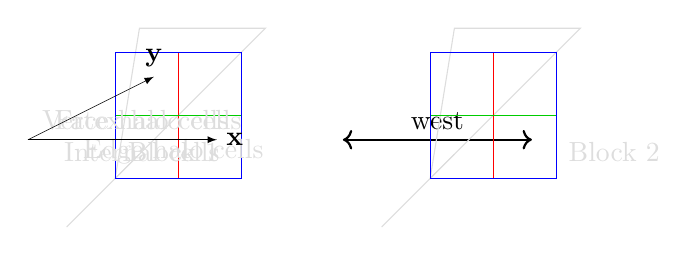
\begin{tikzpicture}[scale=0.8]
        % Define colors
        \definecolor{blockcolor}{HTML}{DDDDDD}
        \definecolor{vertexcolor}{HTML}{FF0000}
        \definecolor{edgecolor}{HTML}{00CC00}
        \definecolor{facecolor}{HTML}{0000FF}

        % Draw block 1
        \draw[blockcolor] (-1,-1,-1) -- ++(2,0,0) -- ++(0,2,0) -- ++(-2,0,0) -- cycle;
        \draw[blockcolor] (-1,-1,-1) -- ++(0,0,2) -- ++(0,0,-1) -- ++(0,0,-2) -- cycle;
        \draw[blockcolor] (-1,-1,-1) -- ++(2,2,0) -- ++(0,0,-1) -- ++(-2,0,0) -- cycle;

        % Highlight halo cells
        \draw[vertexcolor] (-1,-1,-1) -- ++(1,0,0) -- ++(0,2,0) -- ++(-1,0,0) -- cycle;
        \draw[edgecolor] (-1,-1,-1) -- ++(0,1,0) -- ++(2,0,0) -- ++(0,-1,0) -- cycle;
        \draw[facecolor] (-1,-1,-1) -- ++(2,0,0) -- ++(0,2,0) -- ++(-2,0,0) -- cycle;

        % Block 1 labels
        \node[blockcolor] at (0.5,0,0.5) {Block 1};
        \node[blockcolor] at (0,0.5,0.5) {Face halo cells};
        \node[blockcolor] at (0.5,0,0.5) {Edge halo cells};
        \node[blockcolor] at (0,0.5,0.5) {Vertex halo cells};
        \node[blockcolor] at (0,0,0.5) {Internal cells};

        % Arrows for halos
        \draw[<->, thick] (3,0,0) -- node[above,sloped]{west} (6,0,0);

        % Draw block 2
        \draw[blockcolor] (4,-1,-1) -- ++(2,0,0) -- ++(0,2,0) -- ++(-2,0,0) -- cycle;
        \draw[blockcolor] (4,-1,-1) -- ++(0,0,2) -- ++(0,0,-1) -- ++(0,0,-2) -- cycle;
        \draw[blockcolor] (4,-1,-1) -- ++(2,2,0) -- ++(0,0,-1) -- ++(-2,0,0) -- cycle;

        % Highlight halo cells in block 2
        \draw[vertexcolor] (4,-1,-1) -- ++(1,0,0) -- ++(0,2,0) -- ++(-1,0,0) -- cycle;
        \draw[edgecolor] (4,-1,-1) -- ++(0,1,0) -- ++(2,0,0) -- ++(0,-1,0) -- cycle;
        \draw[facecolor] (4,-1,-1) -- ++(2,0,0) -- ++(0,2,0) -- ++(-2,0,0) -- cycle;

        % Block 2 labels
        \node[blockcolor] at (7.5,0,0.5) {Block 2};

        % Coordinate axis
        \draw[-latex, very thin] (-2,0,0) -- (1,0,0) node[right] {$\mathbf{x}$};
        \draw[-latex, very thin] (-2,0,0) -- (0,1,0) node[above] {$\mathbf{y}$};
    \end{tikzpicture}
\end{center}

\end{document}